\documentclass[12pt]{extarticle}

%Some packages I commonly use.
\usepackage[portuguese]{babel}
\usepackage{graphicx}
\usepackage{framed}
\usepackage[normalem]{ulem}
\usepackage{amsmath}
\usepackage{amsthm}
\usepackage{amssymb}
\usepackage{amsfonts}
\usepackage{enumerate}
\usepackage[utf8]{inputenc}
\usepackage{float}
\usepackage{gensymb}
\usepackage[top=1 in,bottom=1in, left=1 in, right=1 in]{geometry}
\usepackage{multirow}
\usepackage{caption}
\usepackage{subcaption}
\usepackage[utf8]{inputenc}
\usepackage{physics}

%A bunch of definitions that make my life easier
\newcommand{\matlab}{{\sc Matlab} }
\newcommand{\cvec}[1]{{\mathbf #1}}
\newcommand{\rvec}[1]{\vec{\mathbf #1}}
\newcommand{\ihat}{\hat{\textbf{\i}}}
\newcommand{\jhat}{\hat{\textbf{\j}}}
\newcommand{\khat}{\hat{\textbf{k}}}
\newcommand{\minor}{{\rm minor}}
\newcommand{\trace}{{\rm trace}}
\newcommand{\spn}{{\rm Span}}
\newcommand{\rem}{{\rm rem}}
\newcommand{\ran}{{\rm range}}
\newcommand{\range}{{\rm range}}
\newcommand{\mdiv}{{\rm div}}
\newcommand{\proj}{{\rm proj}}
\newcommand{\R}{\mathbb{R}}
\newcommand{\N}{\mathbb{N}}
\newcommand{\Q}{\mathbb{Q}}
\newcommand{\Z}{\mathbb{Z}}
\newcommand{\<}{\langle}
\renewcommand{\>}{\rangle}
\renewcommand{\emptyset}{\varnothing}
\newcommand{\attn}[1]{\textbf{#1}}
\theoremstyle{definition}
\newtheorem{theorem}{Theorem}
\newtheorem{corollary}{Corollary}
\newtheorem*{definition}{Definition}
\newtheorem*{example}{Example}
\newtheorem*{note}{Note}
\newtheorem{exercise}{Exercise}
\newcommand{\bproof}{\bigskip {\bf Proof. }}
\newcommand{\eproof}{\hfill\qedsymbol}
\newcommand{\Disp}{\displaystyle}
\newcommand{\qe}{\hfill\(\bigtriangledown\)}
\setlength{\columnseprule}{1 pt}
\usepackage[utf8]{inputenc}

\title{Aula 20 - Conceitos de Física Moderna}
\author{Felipe Salvador}
\date{Atualizado em \today}

\begin{document}

\maketitle

\section{Introdução}
Nessa aula, iremos ver os principais conceitos físicos desenvolvidos a partir do século 20, de forma informal. Ilustraremos descobertas importantes, tais como a relatividade restrita, mecânica quântica e a compreensão de como funciona um átomo, além de escrever as principais equações formadas durante esses estudos. Por fim, como algo extra, falaremos sobre as principais linhas de pesquisa em física e como esses conceitos se tornaram a base para a compreensão dessas áreas.

\section{Albert Einstein e a Teoria da Relatividade}
A partir do final do século 19, alguns problemas com a teoria de Newton sobre a mecânica começaram a aparecer. O principal problema era quando os corpos estavam se movendo a altas velocidades, a teoria conseguia explicar o comportamento dos corpos. Esse era o indício de que algo faltava na teoria de Newton e que tínhamos chegado no limite de validade da teoria.

Durante o mesmo século, os estudos sobre o eletromagnetismo também apresentavam um problema: quando eu mudava o referencial de observação dos problemas, os resultados não batiam. Sabemos que a natureza (clássica) não dá 2 possíveis resultados para um mesmo fenômeno, então algum desses resultados deveria estar errado. Com isso, começou-se então as discussões sobre \textbf{referenciais privilegiados} - referenciais em que os resultados obtidos eram os corretos.

Mesmo durante essa época, os cientistas não estavam convencidos de que a Natureza só possuia um referencial inercial que pudesse explicar corretamente e outros estudos continuaram a serem feitos. Na virada do século, um grupo de físicos e matemáticos começaram a discutir sobre uma transformação, hoje chamada de \textbf{Transformação de Lorentz}, em que  conseguia fazer os resultados do eletromagnetismo, em diferentes referenciais, serem iguais. Logo, o problema de referenciais no eletromagnetismo foi resolvido, mas logo após, em 1904, Albert Einstein deduziu a Teoria da Relatividade, usando as transformações de Lorentz.

A teoria de Einstein parte de 2 postulados (verdades indiscutíveis):
\begin{itemize}
    \item As leis da Física são as mesmas em todos os referenciais inerciais em relação a um outro referencial inercial;
    \item Em qualquer referencial inercial, a velocidade da luz é igual à 'c' ($c=3.10^8\,m/s$).
\end{itemize}

Esses 2 postulados de Einstein são a pedra fundamental da sua teoria e com ela, por meio das transformações de Lorentz, pudemos entender como a natureza se comporta quando aproximamos à altas velocidades. Nós vamos nos ater ao movimento em 1 dimensão (x) + o tempo. Com isso, para um referencial (R') se movendo com velocidade $v$ em relação a um outro referencial (R), a coordenada $x'$ e o tempo (t') no referencial R' se relacionam com as quantidades no referencial R da seguinte forma:
\begin{align}\label{eq:rel_restrita1}
    x' = \gamma(x -vt)\quad \quad \left(\gamma = \frac{1}{\sqrt{1-\left(\frac{v}{c}\right)^2}}\right)
\end{align}
\begin{equation}\label{eq:rel_restrita2}
    t' = \gamma(t-\frac{vx}{c^2})
\end{equation}
\noindent em que  (x,t) são a posição e tempo no referencial R, (x',t') são a posição e tempo no referencial R', $v$ é a velocidade que o referencial R' se movimenta em relação ao referencial R, 'c' é a velocidade da luz no vácuo e $\gamma$ é um coeficiente chamado de \textbf{fator de Lorentz}.

Esse fator é sempre maior que 1, em que é o caso que o referencial R' está parado em relação ao referencial R (v=0):
\begin{equation}
    \gamma = \frac{1}{\sqrt{1- \left(\frac{0}{c}\right)^2}} = \frac{1}{\sqrt{1}} =1
\end{equation}

Esse fator ele aumenta, conforme $v$ chega mais próximo de 'c'. Por meio, das equações (\ref{eq:rel_restrita1}, \ref{eq:rel_restrita2}), conseguimos deduzir 2 fórmulas importantes para a relatividade:
\begin{equation}
    L' = \frac{L}{\gamma}
\end{equation}
\noindent em que essa fórmula se chama \textbf{Contração do Espaço}. No referencial em movimento (R'), o objeto será contraído em relação se o objeto estivesse no referencial parado (R). Isso acontece, porque o $\gamma$ é sempre maior que 1, então $L'< L$ e conforme a velocidade entre os referenciais aumenta, mais contraído o objeto fica.
\begin{figure}[H]
    \centering
    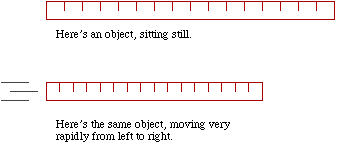
\includegraphics[width=0.6\textwidth]{ruler.png}
    \caption{Contração do espaço numa régua.}
    \label{fig:space_contraction}
\end{figure}

\textbf{A segunda fórmula se chama Dilatação do Tempo:}
\begin{equation}
    \Delta t' = \gamma \Delta t
\end{equation}
Ou seja, conforme a velocidade entre os referenciais aumenta, o intervalo de tempo entre 2 instantes aumenta também, dilatando o tempo. Novamente, isso é possível, porque o $\gamma$ sempre é maior que 1. Então, um relógio no referencial R' anda mais lentamente do que um relógio no referencial parado R. Isso faz com que seja apareça um paradoxo, chamado de \textbf{Paradoxo dos Gêmeos}.

Em 1915, Einstein trouxe a parte mais importante da Relatividade: \textbf{A Relatividade Geral.} Essa teoria afirma que o espaço-tempo é um tecido, em que a massa deforma o espaço-tempo ao redor da massa. Essa teoria consegue explicar muito bem a gravitação (força da gravidade) e foi capaz de explicar o efeito da órbita estranha de Mercúrio. Por meio dessa teoria, foi previsto a existência de \textbf{buracos negros}, por meio do trabalho inicial de Schwarzchild. Só em 2019 conseguimos observar o primeiro buraco negro pelo telescópio Event Horizon Telescope (EHT).
\begin{figure}[H]
    \centering
    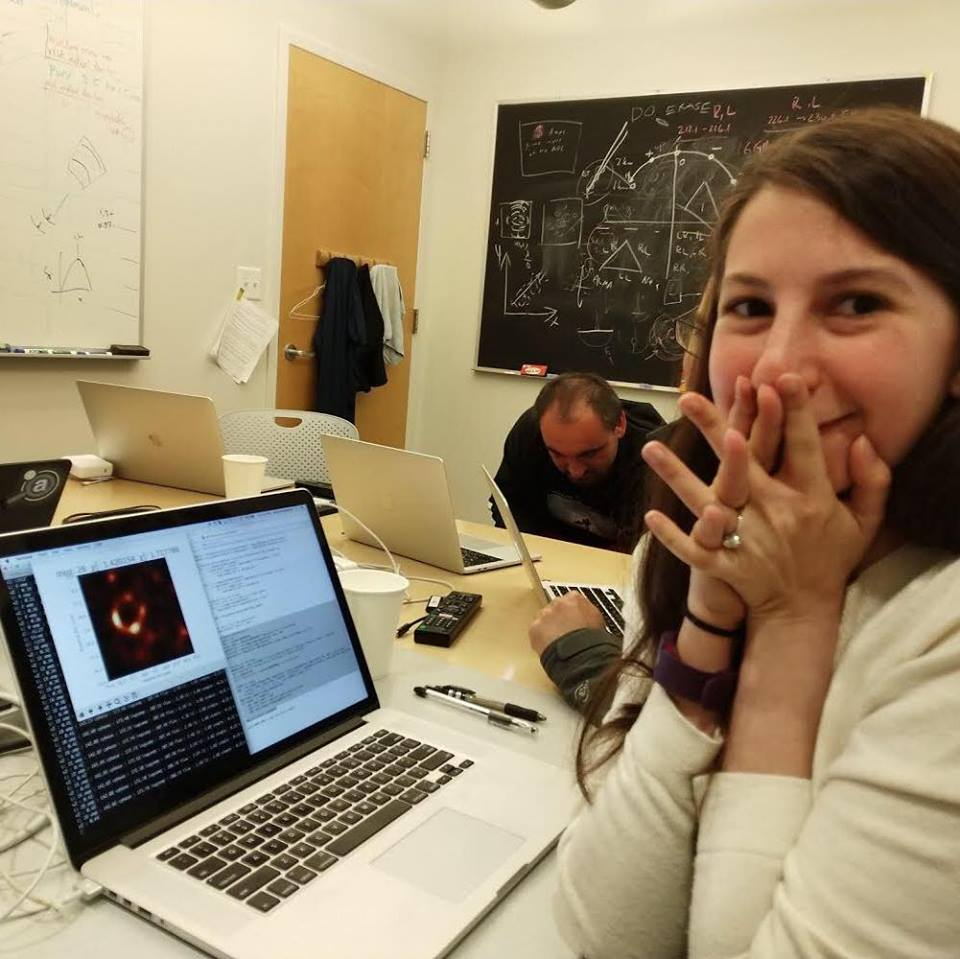
\includegraphics[width=0.6\textwidth]{katie.jpg}
    \caption{Katie Bouman vendo pela primeira vez a imagem do buraco negro. Ela foi uma das pesquisadoras responsáveis pelo código de construção da imagem do buraco negro no EHT}
    \label{fig:katie}
\end{figure}

\section{Teoria e Mecânica Quântica}
Também por volta da virada do século XIX para XX, outras questões estavam em aberta na Física. Uma delas é a chamada \textbf{Catástrofe do Ultravioleta}. Esse problema surgiu nos estudos sobre \textbf{radiação de corpo negro}, que é basicamente o estudo sobre a luz emitida por corpos muito quentes. Percebeu-se que a teoria não conseguia descrever um caráter anômalo que aparecia nos experimentos:
\begin{figure}[H]
    \centering
    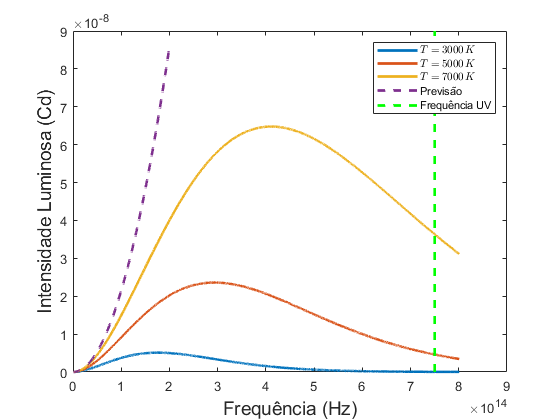
\includegraphics[width=0.8\textwidth]{ultravioleta.png}
    \caption{Catástrofe do Ultravioleta - a teoria clássica do eletromagnetismo não consegue descrever os resultados obtidos, em especial o ultravioleta}
    \label{fig:uv_catastrophe}
\end{figure}

Com isso, começou-se a questionar sobre o que estava por trás desse fenômeno que era inexplicável. A resposta veio 1901, por meio de Max Planck, hoje considerado o Pai da Mecânica Quântica. Ele, por meio da sua explicação, a Lei de Planck, afirma que a energia da luz emitida teria que respeitar uma relação:
\begin{equation}
    E= h\,f
\end{equation}
\noindent em que 'h' é uma constante, a qual chamamos, hoje, de \textbf{Constante de Planck}:
\begin{equation}\label{eq:planck}
    h = 6,62607004 . 10^{-34}\, m^2\, kg / s
\end{equation}
Essa constante é a constante mais importante da Mecânica Quântica (posteriormente desenvolvida ´principalmente por Schrödinger, Dirac, Heisenberg e Hilbert), que aparece em, basicamente todas as contas.

Esse estudo foi o primeiro passo para uma área bem diferente de todas até então, porque durante outros estudos descobriu-se que, na verdade, a frequência emitida pelo corpo negro, não poderia ser qualquer valor, mas um múltiplo de um número base. A isso, se deu o nome de \textbf{quantização}, palavra que vem do latin \textit{quanta}, que quer dizer 'pedaço, fração'. Esse processo todo, agora, impõe restrições para os valores de frequência da luz e, por consequência, para os valores de energia da luz, também.  

Com isso tudo, os estudos sobre corpos negros e átomos fez alavancar o estudo sobre a Mecânica Quântica, a principal área da Física na atualidade. Percebeu-se que os átomos também tem suas energias quantizadas e a teoria fez possível conhecer melhor muitas propriedades, utilizadas em chips, computadores, LEDs e muito mais.

\section{Efeito Fotoelétrico (Einstein)}
Uma das coisas mais interessantes sobre Einstein é que ele não ganhou o Prêmio Nobel de 1921 por causa da Teoria da Relatividade (Restrita e Geral). Na verdade, o trabalho dele sobre Efeito Fotoelétrico é o que rendeu o Nobel de Física e permitiu o desenvolvimento de tecnologias para a captação de energia solar.

Einstein desenvolveu a teoria sobre o Efeito Fotoelétrico que é: Uma onda de luz atinge um material, interage com os elétrons dos átomos, dando para eles energia, e esse elétrons conseguem se despreender dos núcleos dos átomos.

\begin{figure}[H]
    \centering
    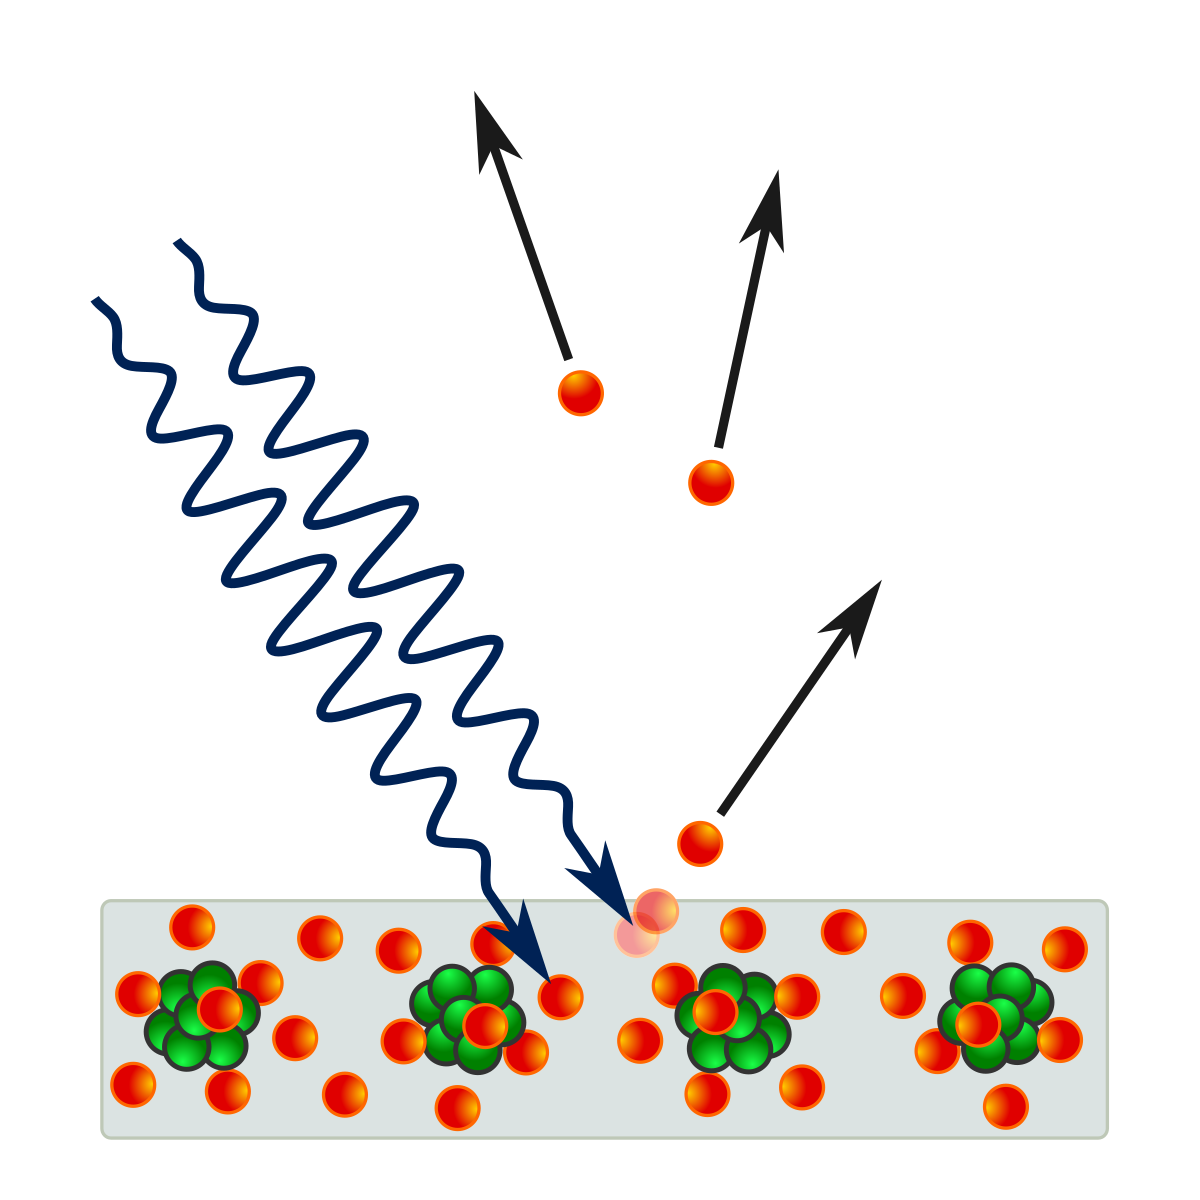
\includegraphics[width=0.6\textwidth]{1200px-Photoelectric_effect_in_a_solid_-_diagram.svg.png}
    \caption{Diagrama do Efeito Fotoelétrico - os elétrons recebem energia da onda de luz, conseguindo escapar dos núcleos atômicos}
    \label{fig:photoelectric}
\end{figure}

Esse fenômeno acontece com mais facilidade quando os elétrons estão nas camadas de valências de átomos metálicos (Sódio, Cobalto, Alumínio, por exemplo). Einstein conseguiu prever a energia que os elétrons escapam a partir de uma simples fórmula:
\begin{equation}
    E_{el}(f) = h\,f + \Phi
\end{equation}
\noindent em que '$E_{el}$' é a energia que o elétron escapa, 'h' é a Constante de Planck (dada na equação (\ref{eq:planck})), 'f' é a frequência da luz e '$\Phi$' é o valor de energia necessária para desprender o elétron do núcleo do átomo. Quanto maior for a frequência da luz, com mais energia o elétron escapará (mais rápido). 

Além disso, uma consequência do Efeito Fotoelétrico é que as contas são feitas tomando a luz composta por partículas chamadas de \textbf{Fóton}. Toda a teoria é feita a partir da colisão entre fótons com os elétrons nos átomos e um fato interessante é que \textbf{os fótons são partículas com massa nula e que anda na velocidade da luz 'c'}. Isso é bem maluco, pois aparenta ir contra a Relatividade de Einstein, mas isso tá dentro das regras, pois a Relatividade só vale para corpos com massa, o que não é o caso dos fótons.

É dessa forma que placas solares funcionam. A luz do Sol atinge a placa e transfere energia para os elétrons da placa, que se desprendem dos seus respectivos núcleos, e formam uma corrente elétrica, alimentando uma bateria. A partir disso, pode-se usar para o consumo de energia elétrica, aquecimento de água de chuveiros e pias, por exemplo.

\section{Átomo de Bohr e Dualidade partícula-onda das partículas}
Até o final do século 19, acreditava que o átomo era composto como o modelo de Thomson descrevia: o modelo do pudim de passas - o átomo era uma grande massa positiva e o elétrons (cargas negativas) estavam dentro dessa massa. Porém, em 1908, 2 físicos - Hans Geiger e Ernest Marsden - conduziram o seguinte experimento:
\begin{figure}[H]
    \centering
    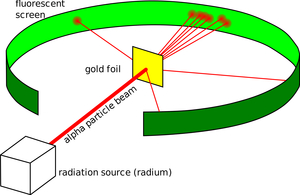
\includegraphics[width=0.7\textwidth]{marsden-geiger.jpg}
    \caption{Experimento de Geiger-Marsden - um canhão que jogava um feixe de partículas alfa ('$\alpha$'), outro nome para o núcleo do átomo de Hélio, na direção de uma fina folha de ouro. Ao redor do experimento, colocou-se uma tela que fluoresce a cada colisão das partículas alfa com a tela.}
    \label{fig:geiger-marsden}
\end{figure}

Pelo modelo de Thomson (Pudim de Passas), esperava que as partículas passassem reto ou, no máximo, desviasse um pouco do centro do feixe. Porém, foi observado algo estranho. Em pontos bem distante do centro, algumas partículas estavam atingindo a tela, algo que não era previsto pelo modelo de Thomson. A partir disso, em 1911, Rutherford propôs um novo modelo: o átomo era composto por um núcleo duro, composto por cargas positivas e onde praticamente toda a massa do átomo estava, e elétrons orbitando ao redor do núcleo, em que os elétrons eram cargas negativas e muito mais leves que o núcleo. A partir do modelo de Rutherford, conseguiu-se explicar os resultados do Experimento de Geiger-Marsden e começamos a adotar o Modelo Planetário de Rutherford para explicar os átomos.
\begin{figure}[H]
    \centering
    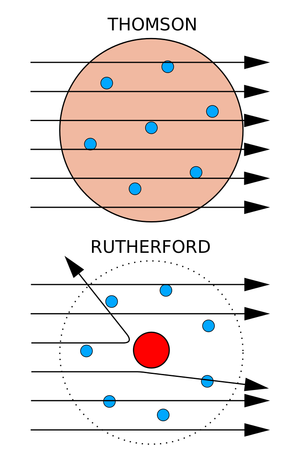
\includegraphics[width=0.3\textwidth]{f2.png}
    \caption{Diferenças nas formas de interação das partículas alfa para um átomo no Modelo de Thomson (Pudim de Passas) e para um átomo no Modelo Planetário de Rutherford.}
    \label{fig:thomson_rutherford}
\end{figure}

Em 1913, Niels Bohr, pupilo de Rutherford, propôs melhorias ao modelo de seu orientador. O modelo Rutherford apresentava um problema: A teoria do Eletromagnetismo previa que os elétrons iriam, depois de um tempo, para no núcleo. Porém, não era isso que era visto na Natureza. Para corrigir esse problema, Bohr colocou 3 postulados (verdades inconstetáveis) que diziam:
\begin{enumerate}
    \item O elétron orbita ao redor do núcleo, sem perder energia por radiação (o que era previsto pelo Eletromagnetismo);
    \item Os elétrons orbitam o núcleo sobre certas órbitas estáveis, que é dado por:
    \begin{equation}
        m\,v\,r = n\,\hbar
    \end{equation}
    \noindent em que 'm' é a massa do elétron, 'v' é a velocidade que ele orbita ao redor do núcleo, 'r' é o raio da órbita (ou a distância do elétron até núcleo) e '$\hbar = \frac{h}{2\pi} \approx 1,0545718.10^{-34}\,m^2\,kg/s$' uma constante chamada de \textbf{Constante de Planck Reduzida} e 'n' é um número inteiro.
    \item Os elétrons ganham/perdem energia na troca de órbitas por meio da absorção/emissão de luz, cuja frequência é 'f' dada por:
    \begin{equation}
        \Delta E = E_2 - E_1 = h\,f
    \end{equation}
    \noindent em que 'h' é a Constante de Planck, $E_2,E_1$ são os valores de energia da órbita que ele está e que ele estava, respectivamente.
\end{enumerate}

A novidade colcada por Bohr foram o $2^\circ$ e $3^\circ$ postulados. Eles diziam as regras que o elétron teria que obedecer enquanto orbita ao redor do núcleo. Ele não pode mais orbitar de qualquer forma, o $2^\circ$ postulado descreve as orbitas que ele pode fazer. O $3^\circ$ postulado diz sobre como o elétron troca de órbita: se ele for para uma órbita com mais energia (uma órbita mais externa), ele tem que ganhar essa energia via luz para pode subir de órbita; se ele for uma órbita com menos energia (uma órbita mais interna), ele tem que ceder energia via emissão de luz para descer de órbita.

Esse trabalho foi o primeiro trabalho sobre como elétrons se comportavam quando rodavam ao redor do núcleo. Mais tarde, por meio da Mecânica Quântica, conseguimos uma descrição mais satisfatória, que estivesse de acordo com outras teorias. Um exemplo de teoria sobre elétrons nos átomos que foi feita por meio da Mecânica Quântica é a Distribuição de Elétrons de Pauli:
\begin{figure}[H]
    \centering
    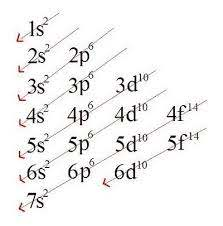
\includegraphics[width=0.3\textwidth]{distribuicao_pauli.jpg}
    \caption{Distribuição eletrônica de Pauli. Ela depende de 3 números quânticos ('n', 'l' e 'm'): $\ket{n,l,m}$. Esse 3 números descrevem o seguinte: 'n' é o 1,2,3,4, ...; 'l' é os 's','p','d','f' e 'm' são os '2','6','10','14',... A ordem de distribuição de elétrons é sempre das órbitas com menos energia para as de maior energia.}
    \label{fig:electron_pauli}
\end{figure}

Estudando mais sobre os elétrons, percebeu-se que eles se comportavam de uma forma bem estranha. A primeira experiência que chamou a atenção sobre isso foi o \textbf{experimento de fenda dupla com elétrons}. Esse experimento é o seguinte: miramos um canhão em direção a uma parede com 2 fendas bem finas e atrás dessas fendas, há uma parede-detector que mede os elétrons chegando. Como os elétrons são partículas, esperamos que aconteça o seguinte:
\begin{figure}[H]
    \centering
    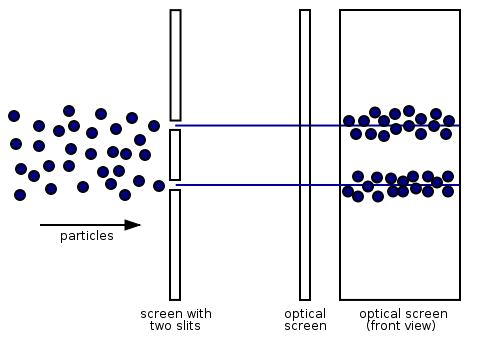
\includegraphics[width=0.5\textwidth]{500px-Two-Slit_Experiment_Particles.svg.png}
    \caption{O esperado para o resultado do experimento}
    \label{fig:expected_double_slit}
\end{figure}

Porém, quando fizeram o experimento, aconteceu o seguinte:
\begin{figure}[H]
    \centering
    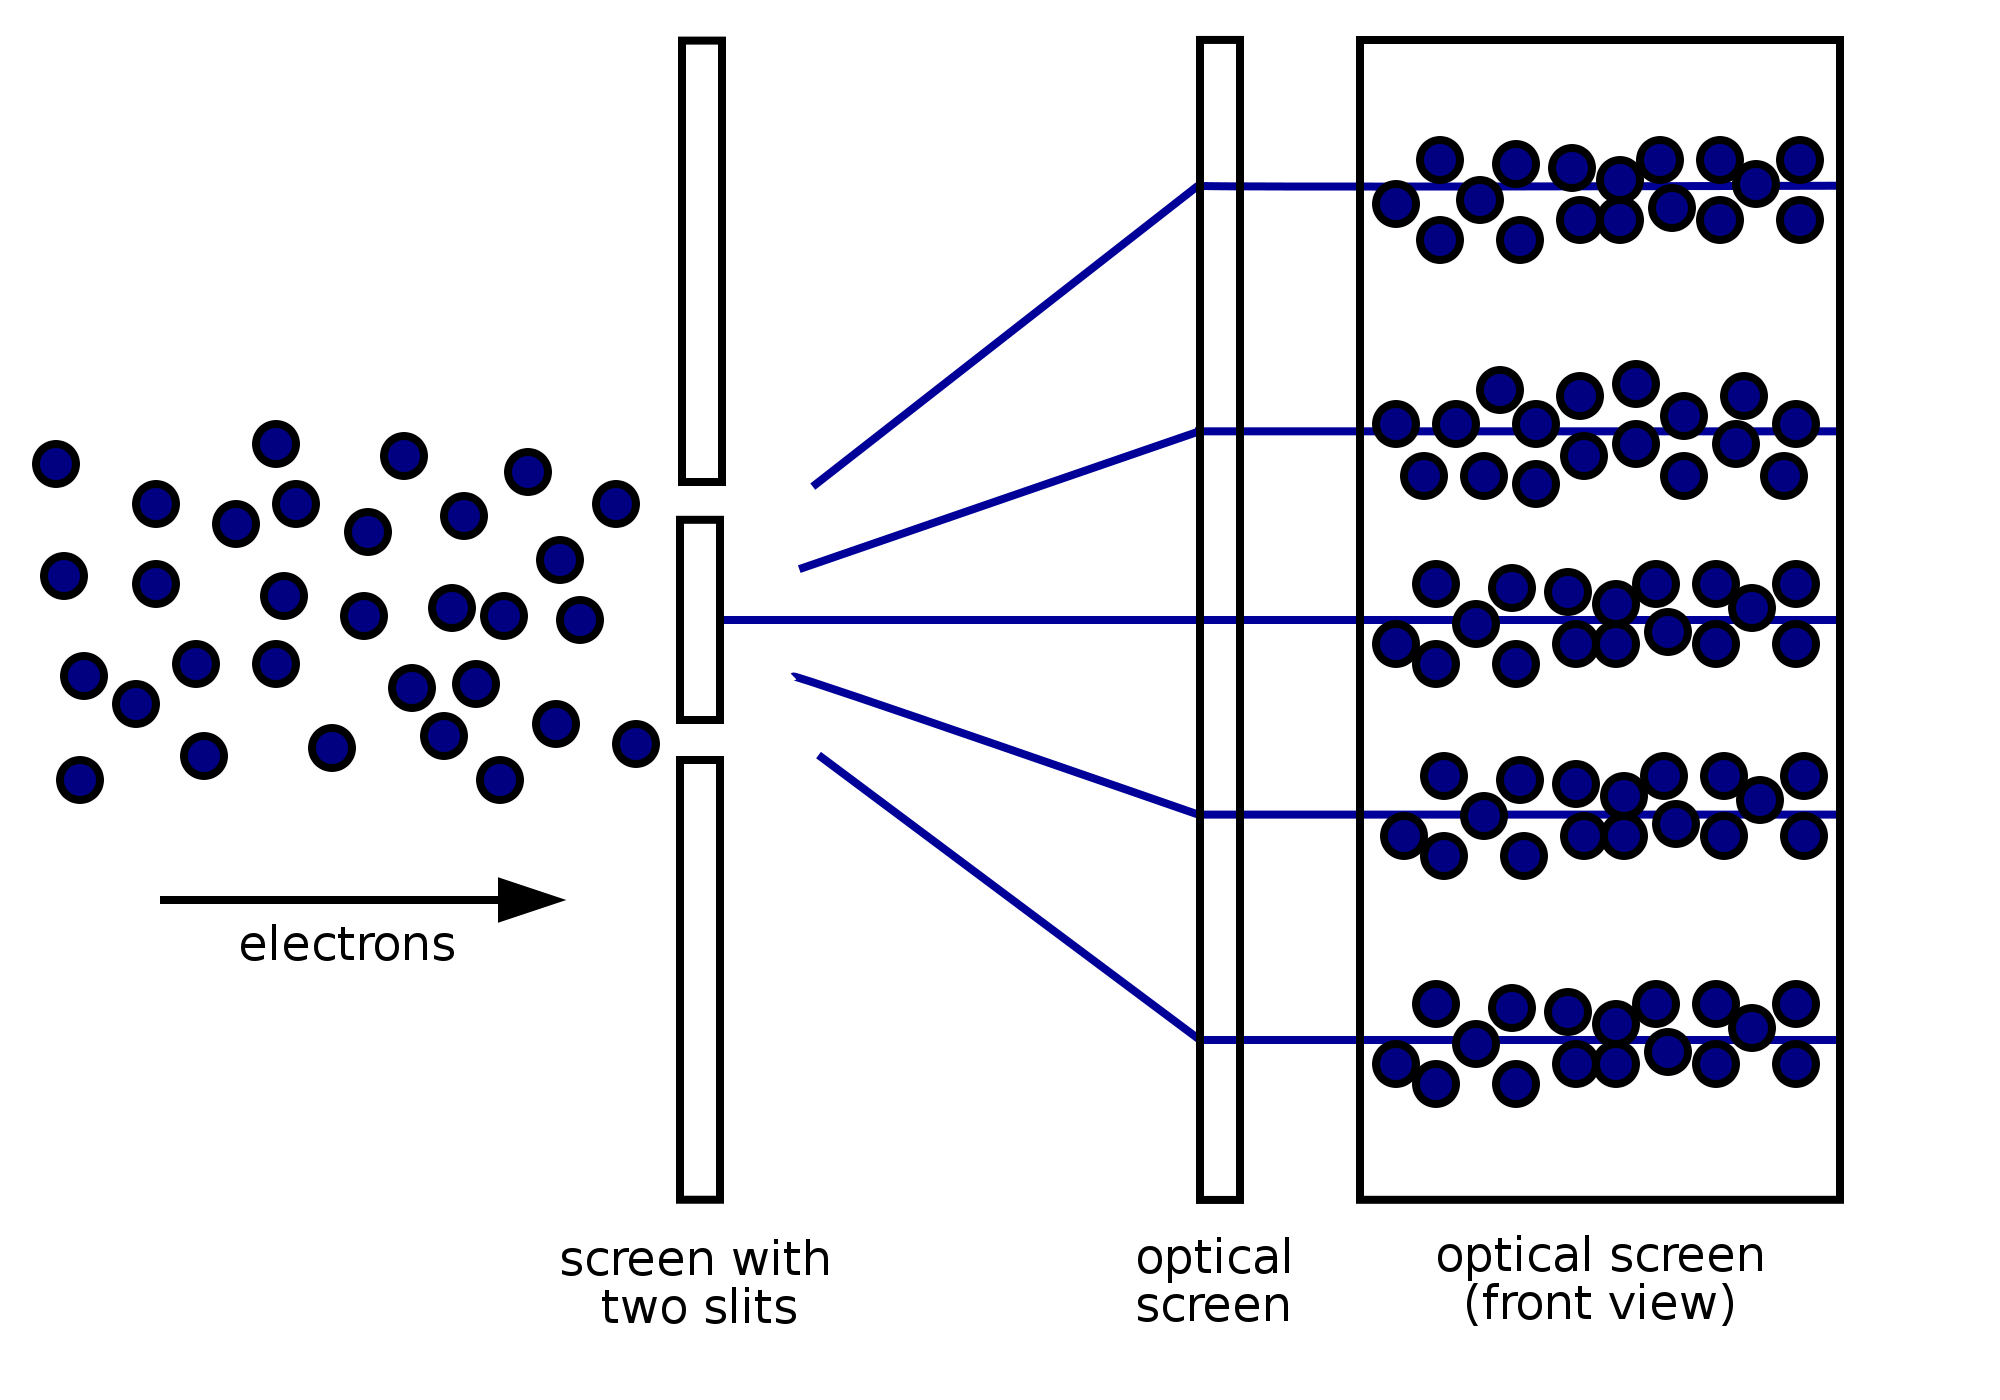
\includegraphics[width=0.5\textwidth]{Double-Slit-Experiment-Results.png}
    \caption{O que foi observado no experimento}
    \label{fig:results}
\end{figure}

Esse resultado, é o mesmo resultado para o experimento feito com luz ou som passando pela fenda dupla: 
\begin{figure}[H]
    \centering
    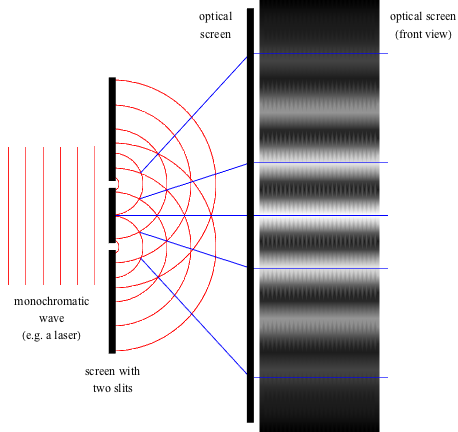
\includegraphics[width=0.5\textwidth]{light_double_slit.png}
    \caption{O resultado obtidos pelo experimento com elétrons é bem semelhante ao resultado obtido com luz, que nem na figura}
    \label{fig:light_double_slit}
\end{figure}

Logo, os cientistas pensaram: ué, o experimento feito com elétrons se comportou como se os elétrons fossem ondas? Não convencidos sobre isso, resolveram instalar 2 detectores na frente de cada fenda. Os detectores sinalizavam quando um elétron passava pela fenda que ele estava medindo. Fazendo o experimento com os detectores, obtiveram o seguinte resultado:
\begin{figure}[H]
    \centering
    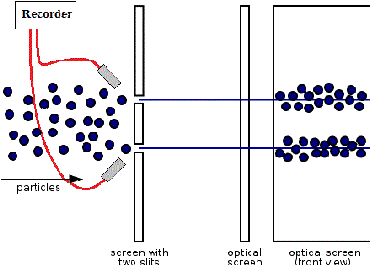
\includegraphics[width=0.5\textwidth]{Two-slit-experiment-with-detector.png}
    \caption{Experimento feito com elétrons, mas agora colocaram detectores na frente das fendas para ver por qual fenda os elétrons passavam. O resultado obtido foi idêntico ao resultado obtido com partículas.}
    \label{fig:detector_double_slit}
\end{figure}

Isso confundiu de vez a cabeça dos cientistas: como que um experimento pode dar um padrão igual à onda e, quando repetimos o mesmo experimento, ele obteve um padrão de partículas. Isso ia contra a crença de que se refazermos um experimento nas mesmas condições, obteremos os mesmo resultados. Mas então, qual foi a saída para isso? Bem, um cara chamado Louis de Broglie, fez um trabalho sobre partículas dizendo: \textbf{Já que a luz se comporta como onda e partícula (fóton), porque a matéria não pode também se comportar como partícula E onda também?}

De Broglie demonstrou por meio da teoria que as partículas atômicas também tem um comprimento de onda associado e esse comprimento é dado por:
\begin{equation}
    \lambda = \frac{h}{m\,v}
\end{equation}
\noindent em que 'h' é a Constante de Planck, 'm' é a massa da partícula e 'v' é a velocidade que a partícula se move.

O resultado obtido por De Broglie é geral. Vale para todas as partículas (com ou sem carga elétrica) e relacionou que a matéria pode ter características de partículas (massa, tamanho, pode colidir, velocidade) como também de ondas (frequência e comprimento de onda). \textbf{Essa relação de que a luz e a matéria se comportam como partícula E onda é chamado de Dualidade Partícula-Onda}.

\section{Principio da Incerteza de Heisenberg}

Werner Heisenberg, um dos físicos que mais contribuiram para o desenvolvimento da Mecânica Quântica, fez um dos trabalhos-chave para o desenvolvimento da teoria: \textbf{O Princípio da Incerteza}. Esse é o primeiro trabalho teórico que impôs limitações das medições de certas quantidades quando estamos observando o mundo quântico. Esse princípio se descreve da seguinte maneira:
\begin{equation}
    \sigma_x\,\sigma_p \geq \frac{\hbar}{2} \approx 5,3.10^{-35}\,kg\,m^2/s
\end{equation}
O que essa equação quer dizer? \textbf{A incerteza na medição da posição de uma partículas vezes a incerteza na medição do momento (p = mv; m - massa da partícula, v - velocidade da partícula) será sempre maior ou igual à $5,3.10^{-15}$}.

Até então, não havia nenhuma lei que impedia os cientistas medirem as coisas exatamente (precisão infinita). Porém, esse trabalho teórico de Heisenberg traz uma incerteza teórica já logo de cara. Isso implica que os cientistas NUNCA conseguirão saber a posição exata e velocidade exata que a partícula está no momento de medição. Isso foi algo único na física teórica e também favoreceu a forma de interpretar a Mecânica Quântica de forma estatística e probabilística.

Assim, nunca teremos a total certeza sobre a posição e movimento de um elétron na órbita ao redor de um núcleo e nem conseguiremos prever qual será o caminho que ele percorrerá. Devido a isso, outros fenômenos bizarros são observados como o caso do \textbf{Tunelamento Quântico}: Esse fenômeno é quando uma partícula pode conseguir se despreender/preender, ao redor da órbita de um núcleo, de forma espontânea, sem receber energia de uma forma externa.

Por causa do tunelamento quântico, a eletrônica de todos os equipamentos eletrônicos funcionam, porque todos esses equipamentos funcionam usando \textbf{transistores}. Os transistores, que são nem portas que medem a passagem de cargas elétricas pela porta, só funcionam porque o tunelamento quântico existe. E dessa forma, foi possível construir chips bem pequenos e cada vez menores para aumentar o processamento sem sermos obrigados a aumentar o equipamento.

\begin{figure}[H]
    \centering
    \begin{subfigure}[b]{0.45\textwidth}
         \centering
         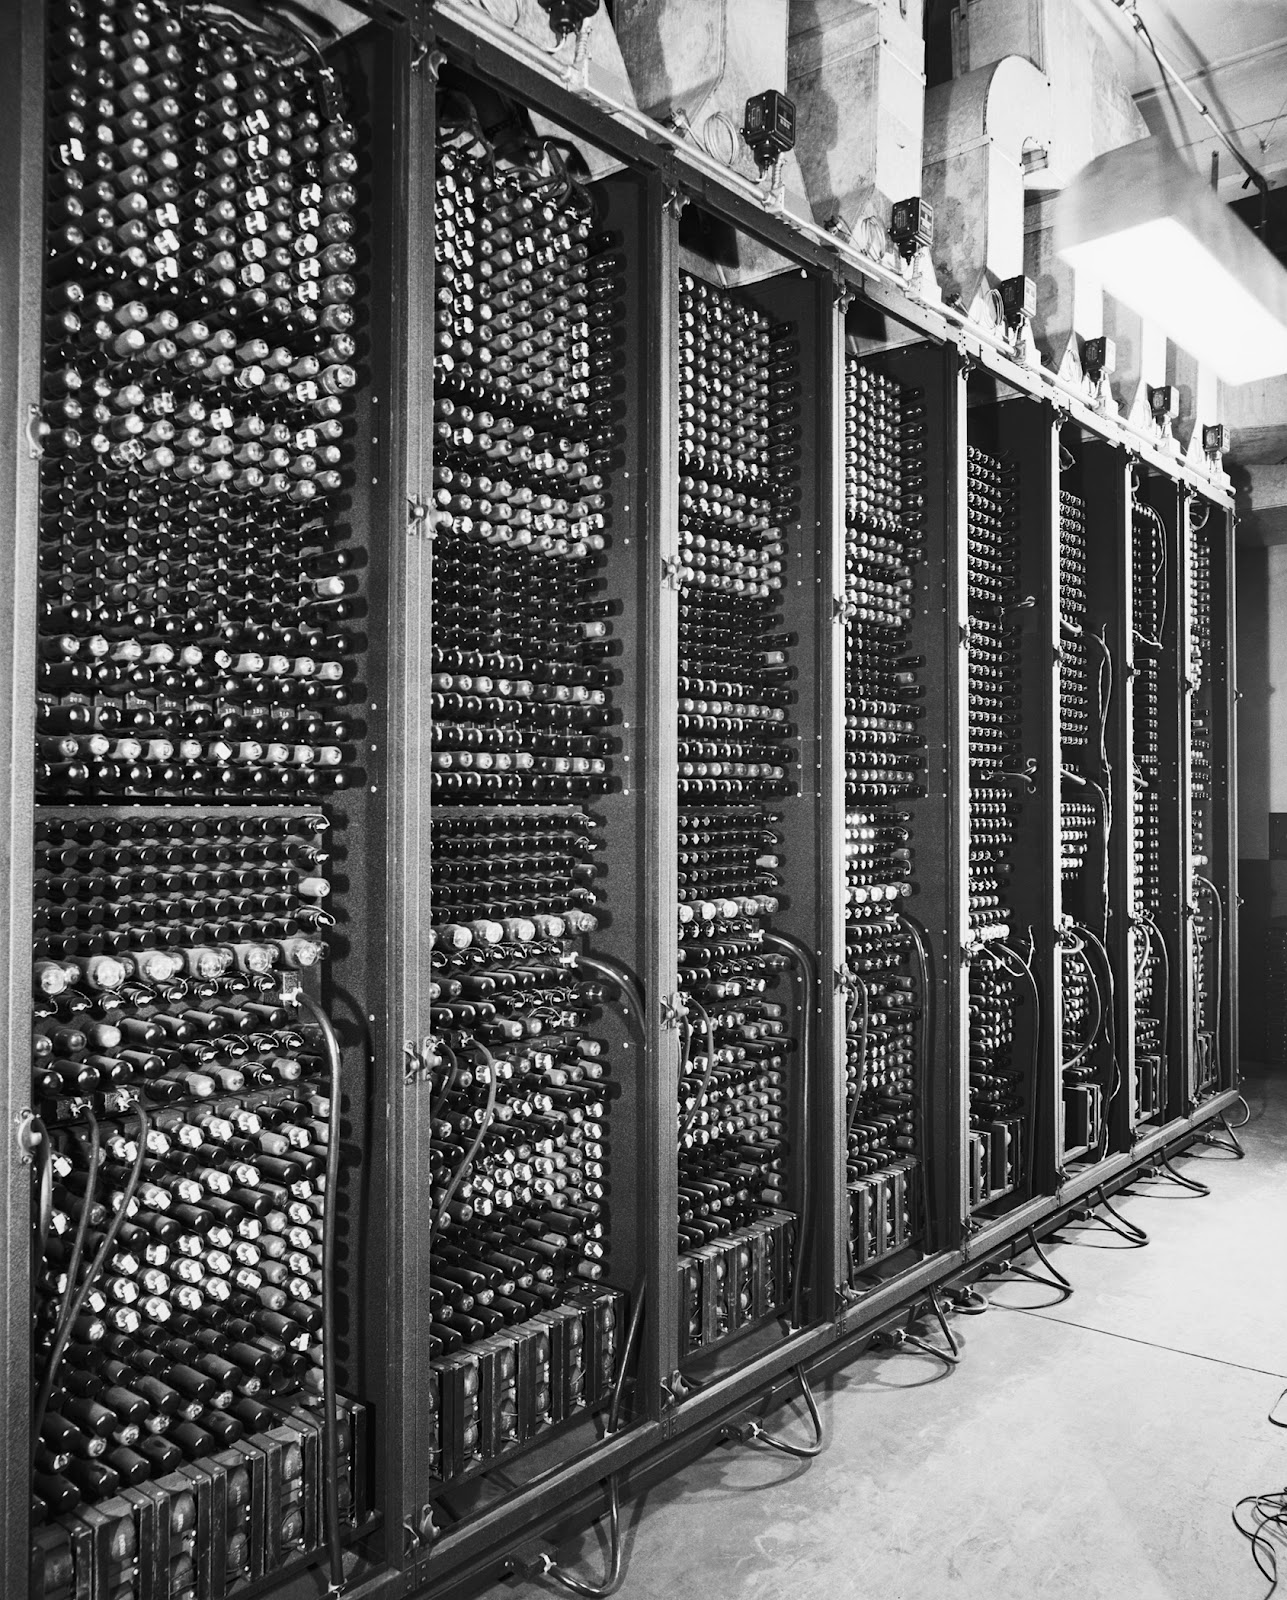
\includegraphics[width=\textwidth]{computador_valvula.jpg}
         \caption{Esse é um computador a base de valvulas eletrônicas, ele ocupava uma sala e o seu carregador de celular tem muito mais poder de processamentos do que esse gigantão ai}
         \label{fig:valvula}
     \end{subfigure}
     \hfill
     \begin{subfigure}[b]{0.45\textwidth}
         \centering
         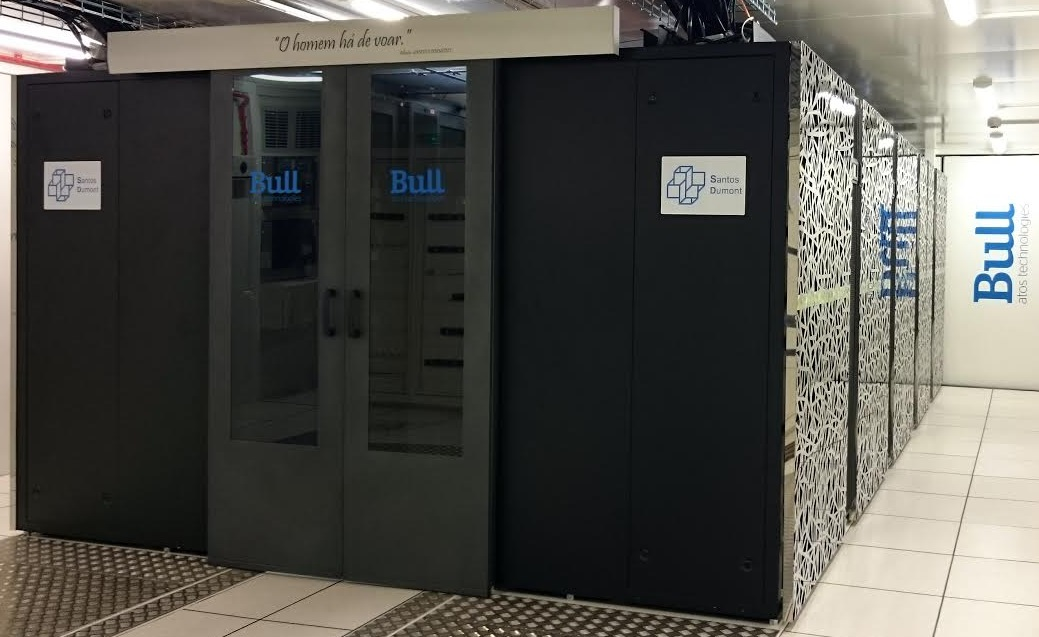
\includegraphics[width=\textwidth]{lncc.jpg}
         \caption{Esse é supercomputador Santos Dumont. Ele fica no Laboratório Nacional de Ciência da Computação em Petrópolis/RJ. Ele é o maior supercomputador do Brasil, capaz de rodar simulações de alta complexidade e processar $5,1.10^{15}$ operações por segundo.}
         \label{fig:santos_dumont}
     \end{subfigure}
     \caption{O quanto evoluimos em menos de 130 anos em termos de processamento. Tudo isso graças ao desenvolvimento do transistor!}
    \label{fig:lncc}
    
\end{figure}
\end{document}
